\chapter{Details of the Microsoft study}
\label{app:Microsoft}

In section \ref{sec:Microsoft} I present some information of the Microsoft study. We published these findings in the proceedings of the 2009 International Conference on Software Engineering \cite{Aranda2009}. The following text is an adaptation of fragments of that paper, included here for completeness.


\section{Motivation}

Modern large-scale software development demands managing huge quantities of bugs on a daily basis. Fixing them is one of the most common and time consuming activities of developers. When bugs number in the thousands, it is unfeasible for both team members and researchers to keep their details present in their minds. Abstraction becomes necessary: project health is measured by bug counts, for instance, and productivity by the rate of bugs closed.

Amid such abstractions it is easy to forget that every bug has a story behind it. The people that discover and resolve it need to coordinate, to get information from documents, tools, or other people, and to navigate through issues of accountability, ownership, and organizational structure. There are awareness requirements, inefficiencies, and opportunities for improved productivity and quality at every step in the process, yet these only become apparent when we go beyond the abstracted numbers and into the rich, detailed history of coordination in each bug.

As researchers, we often rely on repositories of software project information as the main or only source of evidence to extract the histories of bugs and other work items. They are usually stored in the form of tickets or records in a bug database. They provide a convenient compartmentalization of work. We use project management systems' features such as audit trails and data fields that keep track of ownership and of the context of each work item. Sometimes we enrich the histories in ticketing systems with records of electronic communication among team members, and with organizational structure data extracted from human resources databases. However, to this point the use of these electronic repositories as reliable and sufficient accounts of the history of bugs or work items has not been properly validated, and we do not have a description of the common coordination dynamics underlying bug histories.

Our paper reports on a field study of coordination activities around bug fixing that used a combination of case study research and a survey of software professionals. The study goes beyond the electronic repositories of software activity by talking directly to the key actors on the bugs to discover the patterns of group work that are commonly used to fix bugs. It discusses the reliability of electronic repositories as the basis of research into the coordination of software projects, and provides some implications for the design of coordination and awareness tools.


\section{Design and execution}
\label{sec:MicrosoftDesign}

The goal of our study was to provide a rich, contextualized, work-item-centric account of coordination in bug fixing tasks. We had two main research questions:

First, how is the process of fixing bugs coordinated in software teams? What is the lifecycle of bugs? What are the most common patterns of coordination involved in this work? How does their resolution play out over time and over the socio-technical network of the teams that work on them? Second, do electronic traces of interaction provide a good enough picture of coordination, or is non-persistent knowledge necessary to understand the story of each bug fix?

We executed a field study in two parts. The first was a multiple-case exploratory case study of bug histories. The second aimed to validate our case study findings with a survey of software professionals (developers, testers, and program managers). In both cases our data comes from software development at Microsoft's product divisions.

The unit of analysis of our case study was the history of a closed bug. We defined it as the collection of conceptually related activities that at some point in the life of their project were summarized as at least one entry in a bug database. Some records in bug databases are not bugs in the strict sense; we still treated them as such since our teams did. Some bugs have duplicate records; we considered all of the duplicates as part of the same conceptual entity. Some bugs exhibit symptoms that are initially seen as different bugs and recorded separately; we treated them as part of the same defect whenever possible. Bugs do not necessarily begin their life when the entry is created in the bug database or end when they are marked as ``Closed.'' Some of them extend further in both directions; this extended life is part of our unit of analysis. We selected our cases from three major product divisions at Microsoft. Our selection criteria were:

\begin{itemize}
\item The bug was filed in a bug database, and some elementary information about its nature was posted in its data fields.

\item The bug was marked as ``Closed'' at the start of our observations.

\item The bug was fresh (it was closed within two weeks of the start of our observations).
\end{itemize}

Our cases were selected randomly. Other data, such as the bug's resolution mechanism, were not part of our selection criteria, and we did not control for them. To get a better picture of the path that user-reported bugs follow, we deviated from our selection criteria in one case: we contacted a Customer Support escalation engineer and requested a pointer to a bug that had come from Microsoft's escalation channels (that is, a bug that was reported by a customer to support staff).

All of our cases followed the same methodology. First, we queried a product division's bug database to find a case fulfilling our criteria. We obtained as much information as we could from its electronic records, including the events in its audit trail, all the bug record's data fields, data on its owners and on everybody that had participated in any action related to the bug, and links to source code repositories. From that point, we traced backwards by contacting the people that had last touched or were referenced by the bug record. If they were not relevant to the history (a common case, due to bulk edits of bugs), we kept tracing back to find agents that were relevant for the bug.

Once found, we interviewed them to get their understanding of the history of the bug and of the participants and artifacts from which they obtained information or with which they coordinated to close it. When we were pointed to an artifact, such as a specification document, we analyzed it and traced back to its creators. When we were pointed to other people, we contacted them if possible, and repeated the process with them. When we were pointed to a persistent communication medium, such as an email, we obtained a copy, analyzed it, and traced back to its originators.

In some cases this process would reach a dead end but we knew there was more information to be found (because, for instance, we had yet to reach the point where the bug had been originally discovered). If that was the case, we jumped to the next relevant participant in the bug record and continued reconstructing the bug history from that point. We always made sure to reach the beginning of the story.

In other cases our inquiries would lead us to people and artifacts so far along the chain of events that they had little or no relevance to our bug's history. In those cases we made a subjective judgment call and stopped exploring those branches.

Our methodology was theoretically inspired in the focus on people, artifacts, and information flow of Hutchins' \shortcite{Hutchins1995} Distributed Cognition framework. However, as we had expected \cite{Aranda2006}, we found so many instances of information flow that executing our case studies at the computational and representational level of Hutchins' studies was not feasible. We tried to strike a balance between richness and contextual detail on one hand, and replication and generalization power on the other. We stopped collecting data on a chain of events when we had reconstructed it in full, or when we had reconstructed it partially, but proceeding further was unfeasible due to a lack of participation from some of its actors or due to our time constraints.

Our data collection was semi-structured. For each case we collected the following information:

\begin{itemize}
\item A list of primary and secondary actors in the history and their contributions.

\item A list of relevant artifacts and tools.

\item A chronological list of the information flow and coordination events in the bug's history.

\item Pieces of evidence as required by the particularities of each case.

\item The history of the bug as reconstructed by its record in the bug database.

\item The history of the bug as reconstructed by the full collection of electronic traces we obtained.

\item The history of the bug as reconstructed from making sense of all available evidence, including our interviews with participants.
\end{itemize}

In total, we studied ten bugs (including the escalation case). We interviewed 26 people. A brief summary of our cases is provided in table \ref{tab:MicrosoftCases}. Direct Agents are those who executed tasks in the process of resolving the bug; Indirect Agents were addressed by Direct Agents, but did not intervene.

We validated our case study results with a 54-question survey of software professionals at Microsoft. We sent it to 1,500 randomly selected Microsoft employees divided evenly between developers, testers, and program managers. We offered participants a chance to win a \$500US gift card. We received 110 responses (7.3\% response rate); all responses were optional but for all questions we received at least 100 responses. We did not control for the product division of the respondents or for demographic criteria.

The survey asked each respondent about the history of the last recently closed bug that they had played a primary role in resolving. It asked them to go over the corresponding record in the bug database and to bring up and re-read any emails pertaining to the bug, so as to have the history of the bug fresh in their minds.

The survey had three main parts. In the first, respondents gave us general data about the bug in question. In the second we questioned about coordination patterns. In the third, we probed the extent to which the record in the bug database told the full story of their bug.

Results from some of the general data questions appear in Figures \ref{fig:HowFound}, \ref{fig:KindBug}, and \ref{fig:HowClosed}. Although it is not appropriate to compare the case studies with the survey responses using statistical means, the two are mostly in agreement, with one exception: the number of direct agents identified in the case studies versus those reported in the survey. The quartiles for directly involved agents in the survey are 3 (25\%), 4 (50\%), 6 (75\%) and 15 (100\%). In contrast, three of our ten cases had more than 15 directly involved agents. We believe the difference suggests that our investigation revealed a much bigger bug footprint than our respondents perceive.


\begin{figure}[tbp]
\centering
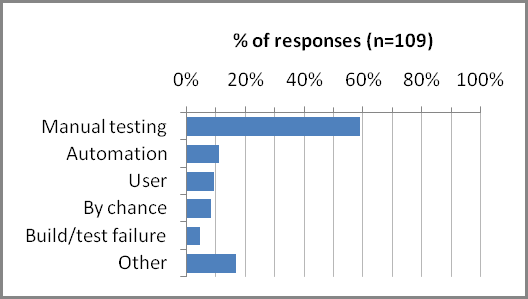
\includegraphics[scale=0.6]{howfound}
\caption{\label{fig:HowFound}Microsoft Study: How was this bug found?}
\end{figure}

\begin{figure}[tbp]
\centering
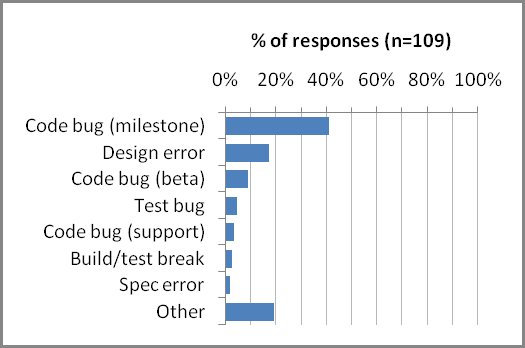
\includegraphics[scale=0.6]{kindbug}
\caption{\label{fig:KindBug}Microsoft Study: Kind of bug}
\end{figure}

\begin{figure}[tbp]
\centering
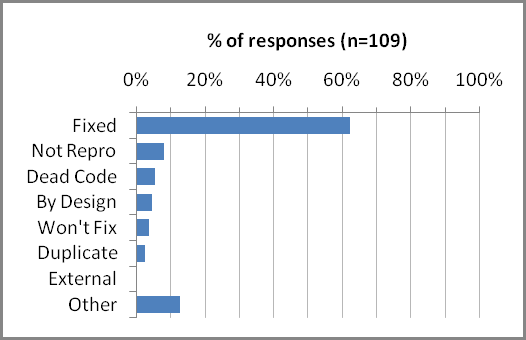
\includegraphics[scale=0.6]{howclosed}
\caption{\label{fig:HowClosed}Microsoft Study: How was this bug closed?}
\end{figure}


\section{Results and observations}

\subsection{Errors and omissions}

The most striking lesson from our cases is the deep unreliability of electronic traces, and particularly of the bug records, which were erroneous or misleading in seven of our ten cases, and incomplete and insufficient in every case. In fact, even considering all of the electronic traces of a bug that we could find (repositories, email conversations, meeting requests, specifications, document revisions, and organizational structure records), in every case but one the histories omitted important details about the bug. Before discussing the errors and omissions in these cases, we need to note that we believe this problem is not a consequence of a carelessness or lack of discipline particular to Microsoft. The repositories and documents we reviewed seem to be as thorough as those of comparable companies, or more.

We found there are several levels at which one can investigate the history of bugs, roughly corresponding to the amount of time one needs to invest in each of them. Each level incorporates all of the information acquired in the previous, plus additional findings from a deeper analysis:

\textbf{Level 1: Automated analysis of bug record data.} At the first level, one can use automation to obtain a list of agents that were involved in a bug's history, as well as information such as a bug's lifespan, its resolution, its changes of state, how was it found, who were its owners, which code change-sets correspond to the bug, and a chronological list of its events.

\textbf{Level 2: Automated analysis of electronic conversations and other repositories.} Traces of electronic conversations can be used to construct a social network of electronic interaction, and assume that it corresponds in structure and intensity to the real communication events of the participants. These data can be filtered by participants, keywords and timestamps to locate the electronic interactions that are (probably) related to the bug in question.

\textbf{Level 3: Human sense-making.} Automation is still far short of a human's capability to infer every connection in the data and reason about the evidence. First, there is often a wealth of information in the electronic repositories described above, but it is not formally linked�discovering it requires a semantic, unstructured analysis of the evidence. For instance, a note by person A in a bug record could state that a fix ``will not address group X's performance concerns, which will be filed in a separate bug.'' An adequately motivated human could conclude that there probably was a discussion between A and representatives of X, extract the list of people that are part of group X from a different database, match it with email records to identify the relevant conversation and agents involved, and, through trial-and-error queries (since no bug ID is provided), locate the follow-up bug in the database. Second, and posing an even greater challenge for automation, if we want to understand and improve coordination dynamics we need our bug histories to include the social, political, and otherwise tacit information that is also part of the bread and butter of software development. This is often subtle, not always apparent, and it must be read between the lines of the evidence collected.

\textbf{Level 4: Direct accounts of the history by its participants.} Interviewing the participants of a bug history seems to be the best gateway to obtain the information that was not documented, or it is disconnected, or erroneous. Interviews enrich significantly the data of the previous levels, as long as they take place before the history of the bug is forgotten. Although they are not guaranteed to provide us a complete account of the bug's history, they allow us to validate earlier conclusions, and to detect events that are not stored in the records, but that are essential to understand it.

We conducted our case study at the last of the four levels we listed. However, throughout its execution, we kept parallel bug histories corresponding to every previous level of analysis of the evidence, in an effort to determine how much of the real histories of bugs is gained or corrected at each level.

The differences between levels were stark, quantitatively and qualitatively. Tables \ref{tab:MicrosoftEvents} and \ref{tab:MicrosoftAgents} help to contrast them. Table \ref{tab:MicrosoftEvents} shows the number of events we could log, for each level, in the bug histories. Similarly, Table \ref{tab:MicrosoftAgents} shows the total number of agents (direct and indirect) found at each level.

Although the numbers support our claims, they cannot show the extent to which the bug histories diverge among levels. It is not just that higher levels produce longer stories; rather, they change qualitatively in ways that are deeply relevant to the study of coordination. The following paragraphs describe the most important kinds of divergence that we observed.

\textbf{Erroneous data fields.} Basic data fields in bug records were sometimes incorrect. C9 was a Test bug, but it was marked as a Code bug. Some duplicates of C2 and of C4 had the wrong Status (they were still marked as ``Resolved'' when their duplicates had been marked as ``Closed''). C8 was resolved as ``Won�t Fix,'' when it should have been resolved ``By Design.''

Our survey asked participants regarding about the Resolution field of their bugs, and their responses support our finding. 10\% of the respondents stated that the Resolution field of their bug was inaccurate.

\textbf{Missing data in bug record.} Among the important bits of data missing from bug records were links to the source code repository in C7 and C10, links to duplicate and related records of bug C2, links to a bug that was found in the process of resolving the original in C9, any links to specification documents (especially for case C5, resolved By Design), reproduction steps (C3), a statement of the corrective actions taken to fix the bug (C2, C4, C7), and a statement of the root cause of the bug (C7, C9).

The missing link to source code change-sets is one of the most problematic omissions. For the last bug of 70\% of our survey respondents, the fix involved committing code to a repository. But 23\% of those cases had no link from the bug record to the source.

The survey supports the rest of our findings too. Reproduction steps were marked as incomplete, inaccurate, or missing, 18\% of the time. Corresponding percentages for the root cause of bugs and the corrective actions taken are 26\% and 35\%.

\textbf{People.} Obtaining the lists of primary and secondary participants in a bug's history was a constant source of errors and omissions. People that took actions concerning the bug were often not mentioned in the record or in email communications (C2, C3, C7, C9, C10). The purported owners of a bug sometimes had no activities or stake in its resolution (C6, C7, C8, C9). The extent of a participant's contribution was easy to misjudge based on electronic traces: high frequency and intensity of interaction did not imply high level of contribution. And in at least two occasions, the geographic location of our interviewees was incorrect in the employee database.

In the survey, the people marked as ``owners'' of the bug were driving its resolution only in 34\% of the time. In 11\% they had nothing to do with the bug.

Furthermore, according to our responses, in 10\% of the time the primary people that worked on a bug are not easy to spot by looking at the bug record, and in 10\% they do not even appear in the record. The list of people that edited the bug's fields and history includes only some of its primary participants 40\% of the time, and none of them 4\%. Corresponding numbers for secondary participants are 39\% and 38\%. All of the people in the bug's history and fields are fully irrelevant in 7\% of the cases.

\textbf{Events.} It is unrealistic to expect all events related to a bug to be found in its record or through its electronic traces. Naturally, most face-to-face events left no trace in any repository. But in some occasions, the key events in the story of a bug had left no electronic trace; the only way to discover them was through interviews with the participants. At the same time, some events logged in the bug records of all of our cases were noise or junk (for instance, bulk edits and mistakes with their later corrections). The chronological order of events was also problematic: bugs were sometimes resolved even before their record had been created (C7), or closed long after they had been resolved because they had been forgotten by the person that needed to close them (C2, C4).

In the survey, 3\% of the bugs had been discussed at least a month before they were first filed, and an additional 6\% at least a week before being filed.

\textbf{Groups and politics.} As we moved further from the raw data and into broader patterns of coordination, we saw that most of the important information at the team and division levels could only be found through higher levels of analysis. In C4 we found a pocket of people with a culture and practices different than those of their division, in the process of assimilation after an acquisition. The status of a group with respect to milestones and releases bore significant consequences to the kind and speed of the decisions made as new bugs were found (for instance, for C5 the team was undergoing a ``bug bash'' and having face-to-face triage meetings daily; most bugs were only given a minute of air time or less). Sometimes, as in C3 and C7, ownership of a bug falls in a gray zone, and inter-team or inter-division struggles to determine ownership and accountability ensue. These issues usually impact the history of bugs considerably, yet we could not have learned about them without interviewing its participants and paying close attention to the details in the electronic record.

\textbf{Rationale.} Probably the hardest questions to answer without human sense-making and participant collaboration were the ``why'' questions: in C4, why did a developer choose another as a required code reviewer, but a third as an optional reviewer? In C10, why was there no activity in a bug record for weeks after a few bouts of minute-by-minute updates and frantic emails? Why were the Status or Resolution fields in C2, C4, and C8 incorrect? Why in C5 did a triage group conclude that the bug would not be fixed? Why did a tester file a bug, C9, even though she suspected the failure was most likely a false alarm? We found that the answers to these questions, discovered during interviews, would often unlock the whole explanation of the events in the history of a bug.

\textbf{Miscellaneous.} Other facts that could only be found at higher levels of analysis resist categorization, but still tend to be at the heart of a bug's history. In C6, a bug was found independently by a tester and a developer in different groups; the developer produced a fix without knowledge that the bug had been already documented. In C4, a developer committed hundreds of new lines of code to fix a bug shortly after it was found; he did not write them all at a blazing speed, but rather copied them from the code of his old company, now acquired by Microsoft, and ``stitched it'' to the relevant interfaces. In two cases (C3 and C7), early and correct diagnoses were promptly ignored in a flurry of emails to get an urgent bug resolved. In general, the bugs in our case pool had far richer and more complex stories than would appear by automatically collecting and analyzing their electronic traces.

\subsection{Coordination Patterns}

In the end, our bug histories were rich, varied, and context dependent. They did not follow a uniform path or lifecycle. This posed a problem: our first research goal was, precisely, to describe the lifecycle of bugs and the process of fixing them.

Instead of attempting to formulate a process for all bug histories, we chose to describe the menu of coordination patterns that we observed. We selected the patterns that seemed to be the most recurrent and those that occurred rarely but had a great impact in the history of a bug. Tables \ref{tab:MicrosoftPatterns1} and \ref{tab:MicrosoftPatterns2} list them.

Some of the patterns have negative implications. For instance, we saw several cases of ``snowballing threads'' and ``rapid fire email in public'' that were clearly inefficient, yet they seemed to be routine for our participants. The only ``summit'' we observed corresponded to a bug (C3) that was described to us as ``very important'' and ``threatening to move our ship date'' by the release manager in charge. We added one pattern for completeness (video conferences), though we observed no instances of it. Another pattern, ``forgotten,'' was pointed to us by one of our survey respondents; it was not included in our original list.

We asked our survey respondents whether those patterns had occurred for their last bug, and if so, whether they had been essential for the resolution of the bug. Figure \ref{fig:Frequencies} provides their responses. The last column represents the perceived usefulness of a pattern in relation to its frequency.

\begin{figure}[tbp]
\centering
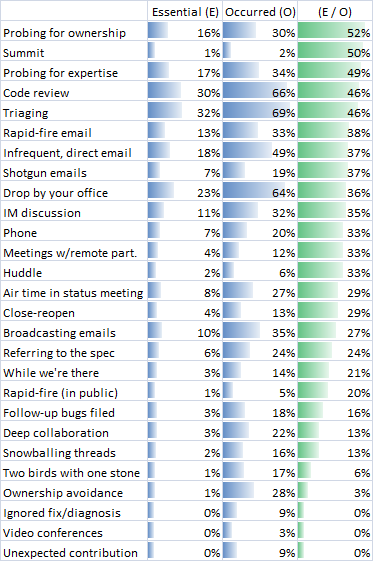
\includegraphics[scale=0.8]{frequencies}
\caption{\label{fig:Frequencies}Microsoft Study: Coordination pattern frequencies}
\end{figure}

We do not claim that our list of patterns is comprehensive. But using them to characterize bug histories may provide enough relevant information about their coordination events while ignoring irrelevant details. Furthermore, some of them could be supported (or in the case of negative patterns, prevented) by software tools.

Although the set of states commonly used in bug databases (Active, Assigned, Resolved, etc.) may be helpful to manage software development, our data shows that they are poor approximations of the true lifecycle of a bug. We believe it is more useful, for understanding coordination and for designing tools for developers, to think of bug fixing activities not as belonging to a stage of a bug�s life or a workflow, but as striving for the satisfaction of one or several goals.

We formulated a list of goals based on the activities of the people in our case study. The following paragraphs describe them. Not all of the goals occur for every case, and they do not occur strictly sequentially.

\begin{itemize}
\item \textbf{Discovery.} Detecting a difference between reality and expectation. The essential first step to record the unexpected behavior as a bug.

\item \textbf{Diagnosis.} Understanding the nature, cause, and impact of the bug, as well as the actions that will be taken as a result. We believe it happens in every case, though often tacitly.

\item \textbf{Assignment of Ownership.} Determining who will be responsible and accountable for the resolution of a bug, both at the group and individual levels.

\item \textbf{Search.} Finding the appropriate knowledge, resources, and skills. It seems to be often meshed with Assignment of Ownership activities, so that the expert is the owner of the bug �but even the owner may need to reach out for other, more specific bits of expertise and knowledge.

\item \textbf{Correction.} What we usually think of as ``fixing a bug.'' Correcting relevant lines of code, changing documentation, scripts, or other artifacts so that reality and expectation match again.

\item \textbf{Closure.} Determining that the organization is willing to live with the current state of things as related to the bug.

\item \textbf{Awareness.} Communicating status to relevant participants. It stretches through the whole history of almost every bug.
\end{itemize}

These goals provide a framework to analyze the effectiveness of coordination and project management tools and practices. For instance, \emph{Assignment of Ownership} is often problematic, especially if there is no clear owner of the seemingly buggy code. In the case study this happened more often with test scripts than with feature code, and with developers leaving their posts without tying loose ends. Tools and practices that ensure that every artifact has an active owner would reduce this problem.

\emph{Search} is another problematic area. In our cases it often resulted in ``snowballing threads'' and ``shotgun emails,'' which sometimes succeed in finding the people or piece of knowledge necessary, but can be extremely inefficient if one considers the person-hours needed by hundreds of email recipients to parse numerous messages that, more often than not, have no relevance for them.

For coordination purposes, \emph{Awareness} was the area most in need of improvement. However, it is not easy to figure out how to provide the right level of awareness in very large companies with interconnected products. Awareness seems to be most needed not at the team level, but among the primary and secondary agents that form the social network around a work item. Tools that (partially) detect work networks and allow for their members to be aware of the activities of their peers should help address this issue.


\section{Limitations}

During our analysis we worked with several concepts that do not yet have a consistent definition in the literature. In particular, one could argue that our coordination patterns and goals are subjective and have blurry boundaries�we never specified, for instance, the difference between ``rapid-fire'' and ``infrequent'' emails. Although this is a valid criticism, our constructs are a first iteration given the data we collected. Additional data and further iterations should refine these constructs, and add others that help convey the underlying concepts more clearly.

Our data come exclusively from Microsoft, and the extent to which our results are valid for other companies is not clear without replications. As is well known, Microsoft has tens of thousands of employees, millions of daily users, and many interconnected products. These are all forces that shape coordination dynamics. However, the use of software repositories and communication media at Microsoft seems to be similar to that of comparable companies. The clearest finding in our study, the difference between the minable version and the true version of a bug's history, should not be Microsoft-specific, as it depends not on corporate culture but on the amount and quality of the information that can be economically and efficiently captured electronically. It is possible that for some software development environments, particularly open source, in which all or most information is communicated electronically and persistently, this is less of a problem. Replications of this study would help resolve that question.